\section{Distance Bounding Protocols}
\begin{figure}
  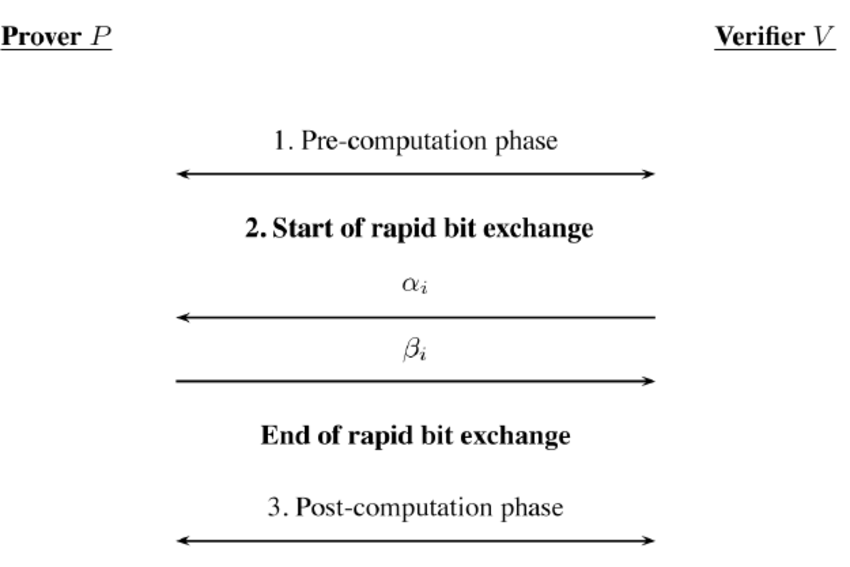
\includegraphics[width=\textwidth]{pictures/distance_bounding.png}
  \caption{A distance bounding protocol~\cite{Peeters2011-bd}.}
  \label{Distance Bounding Protocol}
\end{figure}
Distance bounding protocols are interactive protocols that aim to measure the physical distance or latency between two participants, the prover and the verifier. They are solutions to problems where a simple ping will not suffice, as either party could quite easily craft a false measurement. Distance bounding is used in applications like IP geolocation, wireless access control, and routing in P2P (ad-hoc) networks.

The first distance bounding protocol was designed by Brands and Chaum in 1993 to counter so-called relay attacks~\cite{Boureanu_undated-bn, Brands1994-hz}. A commonly used example of a relay attack is that if the signals between a credit or a debit card and a point of sale system were to be relayed over a distance, two attackers could pay with the relayed info in a totally different country, for example. A distance bounding protocol is safe if information never gets passed faster than the speed of light, and if causality holds due to the prover not being able to create a valid response to a challenge before it has received the challenge~\cite{Boureanu2014-bn}.

The original definition of a distance bounding protocol consisted of three phases: initial phase, critical phase, and a verification phase~\cite{Brands1994-hz, Mauw2018-uz}.

\begin{enumerate}
  \item The Initial Phase --- the two peers agree on the parameters used.
  \item The Critical Phase --- the two peers do multiple challenge/response rounds.
  \item The Verification Phase --- optional, because the verifier can also verify the proofs during the critical phase.
\end{enumerate}

A way to infer physical distance \(d\) from the measured round trip time \(\Delta t\) is to convert the latency to an approximation of the round trip time \(\Delta t\) divided by two times two-thirds the speed of light \(c\)\footnote{Approximation of network transmission speed in optic fiber widely used in IP geolocation~\cite{Candela2020-am}.}:

\begin{equation*}
  d = \frac{1}{2}\Delta t \frac{2}{3}c
\end{equation*}

Even when not using distance bounding for geolocation one can use the aforementioned method to pick sane parameters for each application, like attack prevention in point of sale systems and RFID lock tags. For the measurement to be as close to ground truth as possible, there needs to be sufficient computing power and a good software implementation to minimize any processing delay introduced between receiving the challenge and sending the response, as this delay lowers the maximum measured resolution achieved by the protocol. For point of sale systems, this delay can be crucial, as we only want the point of sale system to be used by the customer right next to it.

When distance bounding is used in other ways than highly local applications like car keys, e.g. in digital rights management, it can reveal too much of the user's location. Usually distance bounding protocols have assumed that both the prover and the verifier are willing to disclose their locations. Some newer protocols have tried to introduce a cloaking region by reducing measurement resolution by adding a delay to the challenge responses.~\cite{Molina-Martinez2018-nw} This is a welcome solution in instances where a verifier only needs to know a rough estimate of the prover's location instead of a tight bound, for example in content delivery networks.

\subsection{Attacks}
Distance bounding protocols were originally invented to solve the problem of relay attacks. These attacks are usually not an issue anymore, and distance bounding is used widely in RFID readers nowadays~\cite{Nikov2008-vv}. There are, however, still potential attacks that could affect distance bounding. Historically, the attacks against distance bounding have been categorized into five different categories~\cite{Boureanu2014-bn}:

\begin{itemize}
  \item \emph{Distance fraud}, where a far-away prover tries to pass the protocol by itself.
  \item \emph{Mafia fraud}, which is a man-in-the-middle attack where a malicious peer in between an honest prover and a verifier tries to get the verifier to accept the far-away prover's proof.
  \item \emph{Terrorist fraud}, where with a help of a temporary adversary a malicious far-away prover tries to make the verifier accept its proof without revealing any secrets to the adversary.
  \item \emph{Impersonation fraud}, where a close-by adversary impersonates a prover.
  \item \emph{Distance hijacking}, where a far-away prover takes advantage of honest provers to make the verifier accept its proof.
\end{itemize}

Inferring from the categories one can deduce that requiring the participants to digitally sign the passed messages in a cryptographically secure manner will render most of these attacks unfeasible, unless, of course, the prover has been hacked or in some other way it has leaked its secrets to a malicious third party.
